\documentclass[conference]{IEEEtran}
\IEEEoverridecommandlockouts
% DRAFT -- every number below comes from results/final/ and results/video/ in the project repository.
% Placeholders that need the authors' input are marked TODO.
\usepackage{cite}
\usepackage{amsmath,amssymb,amsfonts}
\usepackage{graphicx}
\usepackage{textcomp}
\usepackage{xcolor}
\usepackage{booktabs}
\usepackage{multirow}
\usepackage{url}
\def\BibTeX{{\rm B\kern-.05em{\sc i\kern-.025em b}\kern-.08em
    T\kern-.1667em\lower.7ex\hbox{E}\kern-.125emX}}
\newcommand{\todo}[1]{\textcolor{red}{[TODO: #1]}}

\begin{document}

\title{Speech Errors and Screen Text in LLM Summaries of Hinglish Tutorial Videos: A Fact-Level Pilot Study}

\author{
\IEEEauthorblockN{\todo{Author 1}}
\IEEEauthorblockA{\textit{Dept. of CSE (AI\&ML)} \\
\textit{KIET Deemed to be}\\ \textit{University}\\
Ghaziabad, India \\
\todo{email}}
\and
\IEEEauthorblockN{\todo{Author 2}}
\IEEEauthorblockA{\textit{Dept. of CSE (AI\&ML)} \\
\textit{KIET Deemed to be}\\ \textit{University}\\
Ghaziabad, India \\
\todo{email}}
\and
\IEEEauthorblockN{\todo{Author 3}}
\IEEEauthorblockA{\textit{Dept. of CSE (AI\&ML)} \\
\textit{KIET Deemed to be}\\ \textit{University}\\
Ghaziabad, India \\
\todo{email}}
\and
\IEEEauthorblockN{\todo{Author 4}}
\IEEEauthorblockA{\textit{Dept. of CSE (AI\&ML)} \\
\textit{KIET Deemed to be}\\ \textit{University}\\
Ghaziabad, India \\
\todo{email}}
\and
\IEEEauthorblockN{\todo{Author 5}}
\IEEEauthorblockA{\textit{Dept. of CSE (AI\&ML)} \\
\textit{KIET Deemed to be}\\ \textit{University}\\
Ghaziabad, India \\
\todo{email}}
}

\maketitle

\begin{abstract}
Lecture and tutorial videos in India are often in Hinglish, mixing Hindi and English within a sentence, and their automatic summaries depend on speech recognition that handles code-switching poorly. We measure how much summary content survives recognition errors and whether text shown on screen can make up for them. From the MUCS 2021 Hindi-English test set we take 25 five-minute windows of software tutorials and summarise each with one fixed large language model, Qwen2.5-7B-Instruct, from the human transcript, from two recognisers, from transcripts with noise on Hindi-only or English-only words, and from these transcripts combined with OCR text from the matching tutorial videos. A separate language model judges, blind to condition, which of 268 atomic reference facts each summary contains, and a human checks the judge and the references. A generic recogniser (word error rate 0.70) cuts fact recall from 0.47 to 0.21, while a Hinglish-tuned recogniser (0.28) causes no significant loss: much of its English-word error is English written in Devanagari, which the summariser handles without loss. Noise on Hindi words lowers recall more steadily than noise on English words. Adding raw on-screen text lowers recall from a good transcript (0.51 to 0.39) but recovers facts visible on screen when recognition is poor (0.18 to 0.30 with the generic recogniser). Rule-based cleaning of the OCR text roughly halves the loss for the human transcript, a consistent but not significant improvement, and screen text alone recalls only 0.11. The judge agrees with the human on 29 of 30 sampled decisions but only moderately with itself across passes, so subgroup results are preliminary.
\end{abstract}

\begin{IEEEkeywords}
code-switching, Hinglish, speech recognition, multimodal summarization, video OCR, large language models, LLM-as-a-judge
\end{IEEEkeywords}

\section{Introduction}
Much classroom and coaching instruction in India is delivered in Hinglish: Hindi grammar with English technical vocabulary, switching inside a sentence (``ab terminal open karo aur \texttt{gcc} command type karo''). Summarising such recordings automatically usually requires a cascade of automatic speech recognition (ASR) followed by a summariser, and ASR is known to struggle with code-switched speech~\cite{diwan2021mucs,chadha2022}. Recognition errors can propagate into the summary, but how much content is lost, and whether the loss falls on the Hindi or the English part of the speech, has not been measured for Hindi-English audio. Tutorial videos also carry a second channel: the screen shows slide text, commands, and program output, often in English. Whether this visible text can compensate for recognition errors is a natural multimodal question~\cite{palaskar2019how2sum}.

We study this question with a controlled design. One summariser is held fixed and only its input changes: the human transcript (\emph{oracle}), the outputs of two recognisers, transcripts with synthetic errors restricted to Hindi or to English words, and each transcript paired with text read from the matching tutorial video by optical character recognition (OCR), raw or cleaned. Summary content is measured at the level of atomic facts, each tagged by the language of its evidence in the transcript, so that losses can be attributed to Hindi-spoken or English-spoken content, in the spirit of the code-switching loss described by CS-Sum~\cite{suresh2025cssum}.

Our contributions are:
\begin{itemize}
\item A fact-level measurement of how code-switched ASR errors propagate into LLM summaries of Hindi-English speech, with oracle, real-ASR, and language-targeted noise conditions on the same 25 windows.
\item Evidence that word error rate overstates downstream damage: a Hinglish-tuned recogniser writes much English in Devanagari, and a script-shift experiment shows the summariser is insensitive to that script change.
\item A controlled test of on-screen text as a second modality: aligned video OCR recovers facts visible on screen when recognition is poor but costs content when the transcript is good, and rule-based cleaning reduces, without removing, that cost.
\item A validated evaluation protocol: a blind LLM judge with specificity rules, repeated judging passes, and human checks of judge decisions, reference facts, and language tags. We report the judge's limits alongside its agreement with a human.
\item All code, prompts, model outputs, OCR text, and judgements, released for reproduction at \url{https://github.com/ItyGaur/hinglish-asr-summarisation}.
\end{itemize}

To our knowledge no prior work measures this propagation for Hindi-English speech or tests on-screen text as a remedy; we do not claim a new dataset or model.

\section{Related Work}
\textbf{Code-switched summarisation.} GupShup introduced summarisation of Hindi-English chat conversations~\cite{mehnaz2021gupshup}. CS-Sum benchmarks LLMs on code-switched dialogue summarisation for Mandarin, Tamil, and Malay with English, and names code-switching loss, where summaries rely on the English parts and drop content from the other language~\cite{suresh2025cssum}. Both operate on text; neither studies speech input or Hindi-English ASR errors.

\textbf{Hinglish ASR.} The MUCS 2021 challenge released Hindi-English code-switched speech from spoken tutorials~\cite{diwan2021mucs}, and wav2vec~2.0 systems reached 21.77 WER on its blind set~\cite{chadha2022}. Whisper-based models~\cite{radford2023whisper} have since been fine-tuned for Hinglish; the model card of the Trelis checkpoint we use reports 13.67 WER on CoSHE-500 against 29.74 for whisper-large-v3 (self-reported)~\cite{trelis2025}. Token-level code-switching detection for Indic text is an active line of work~\cite{bhanushali2026csdi}; we use a simpler script-share rule (Section~\ref{sec:facts}).

\textbf{ASR errors in downstream tasks.} ASR-GLUE showed that NLU accuracy degrades under ASR errors~\cite{feng2021asrglue}, and MEDSAGE studied ASR errors in medical dialogue summarisation and used LLM-generated noise for augmentation~\cite{binici2025medsage}; both are English-only. Closest to us, Havare et al.\ show that ASR errors in Hindi, Bengali, Tamil, and Gujarati degrade downstream code question answering and retrieval~\cite{havare2026lost}; we study summarisation of lecture-style audio. Applied systems summarise Indian educational lectures with LLM APIs~\cite{kumar2026ccic} but do not analyse recognition errors.

\textbf{Multimodal summarisation of instructional video.} How2 provides instructional videos with transcripts and summaries~\cite{sanabria2018how2}, and multi-source models that combine transcript and video features improve summaries on it~\cite{palaskar2019how2sum}. Those models are trained for the task and use visual features of English videos; we instead give a general instruction-tuned LLM the text that OCR~\cite{smith2007tesseract} reads off the screen of Hindi-English tutorials, and measure what that text adds or removes at the level of facts.

\textbf{Evaluating code-mixed generation.} Surface metrics such as BLEU and BERTScore are unreliable on Hinglish text~\cite{srivastava2021hinge}. We therefore use fact-level evaluation in the style of atomic-fact scoring~\cite{min2023factscore}, judged by an LLM~\cite{zheng2023judge}, and report ROUGE~\cite{lin2004rouge} and BERTScore~\cite{zhang2020bertscore} as secondary metrics.

\section{Data and Conditions}
\subsection{Windows}
The MUCS 2021 Hindi-English test set contains 30 spoken-tutorial recordings (5.18~h) with human transcripts~\cite{diwan2021mucs}. Before any summary was scored, we selected 25 windows with a fixed seed: contiguous stretches of 300--600~s of speech with at least 5\% English and 30\% Hindi tokens, one window per recording after removing near-duplicate recordings. The windows total 126.3 minutes; on average 27\% of their tokens are English.

\subsection{Recognisers}
We transcribe each window with whisper-small and with the Hinglish fine-tune Trelis whisper-hinglish-preview~\cite{trelis2025} (faster-whisper, beam 5, temperature 0, language token \texttt{hi}, voice-activity segmentation into clips of at most 15~s). Table~\ref{tab:asr} gives corpus-level error rates. The two models differ in size as well as in fine-tuning: the Trelis model is built on whisper-large-v3.

\begin{table}[t]
\caption{Corpus-Level ASR Error Rates on the 25 Windows}
\label{tab:asr}
\centering
\begin{tabular}{lcc}
\toprule
 & whisper-small & Trelis \\
\midrule
WER & 0.697 & 0.282 \\
Transliterated WER & 0.659 & 0.260 \\
Hindi-token error & 0.491 & 0.143 \\
English-token error & 0.964 & 0.465 \\
\bottomrule
\end{tabular}
\end{table}

\subsection{Controlled noise and script conditions}
To separate errors on the two languages, we corrupt the oracle transcript on Hindi-only or English-only tokens at injected error rates of 10--50\%. Substitution, deletion, and insertion proportions and the substituted words are sampled from Trelis's real errors on the other 24 windows (leave-one-window-out). Two further conditions test script: \emph{script-shift} rewrites the oracle's English words in Devanagari using a 532-entry lexicon (83\% of English tokens covered), and \emph{back-transliteration} maps Devanagari-written English in the Trelis output back to Latin script, using a lexicon built only from the other windows.

\subsection{Screen text from the videos}\label{sec:screen}
MUCS recordings come from Hindi Spoken Tutorial videos. We matched each window to the earlier, Hindi-narrated version of its video on the Spoken Tutorial site (videos of 343--902~s) and located the window by normalised cross-correlation, at 8~kHz, of 6-s audio templates from its first and last utterances against the video soundtrack. Both ends matched clearly for 17 windows; for 4 the first-utterance match was weak and the start was set from the end match minus the window's speech duration; 4 fell back to a proportional estimate. Within each window's span we sampled one frame every 2~s, kept a frame only when its perceptual hash differed from the last kept frame by more than 6 bits, and read it with Tesseract~\cite{smith2007tesseract} (English, sparse-text mode, frames upscaled 2$\times$, words with confidence above 60), removing duplicate lines. The time-stamped lines form the \emph{raw} screen text (mean 5,356 characters, capped at 6,000).

Raw desktop OCR is dominated by menus, status bars, credits, and fragments. \emph{Cleaned} screen text applies fixed rules, frozen before any cleaned summary was generated: it drops credits, status bars, lines whose words are mostly standard menu names, and lines that are not sentence-like (fewer than four words, or under 75\% dictionary words by word frequency~\cite{speer2022wordfreq}); keeps code, commands, and program output; rejoins bullet lines split by OCR; removes near-duplicates; and caps the text at 2,000 characters. It keeps 1,191 of 6,696 OCR lines (mean 1,170 characters).

Each of the oracle, Trelis, and whisper-small transcripts is summarised together with raw and with cleaned screen text, and the screen text is also summarised alone. A fact counts as \emph{on screen} if at least half of its content words (four or more letters, excluding stop words) occur in its window's raw OCR text; 90 facts in 22 windows qualify and 178 are \emph{speech-only}.

\subsection{Silver references and facts}\label{sec:facts}
From each oracle transcript, Gemini (gemini-3.8-flash) wrote a 120--180-word reference summary and a list of atomic facts, each with an evidence excerpt copied verbatim from the transcript. All 268 facts (10--13 per window) were located in the transcript. Each fact is tagged by the script of its evidence: \emph{hi} if at least 60\% of the evidence tokens are Devanagari, \emph{en} if at most 40\%, and \emph{mixed} otherwise, giving 170 hi, 70 mixed, and 28 en facts. The tag is deterministic and approximates the language of the speech.

\subsection{Summariser}
Every input is summarised by Qwen2.5-7B-Instruct~\cite{qwen2025} (4-bit NF4, greedy decoding, one fixed prompt) into an English summary of 120--180 words. Re-running the model reproduced all 256 previously generated summaries exactly. We also request Hinglish summaries for the oracle and both ASR inputs (Section~\ref{sec:hinglish}). For the screen conditions the same prompt adds one sentence explaining that OCR text from the video follows the transcript, and the screen text is appended after it; screen-only summaries use a prompt that asks for a summary of the screen text alone. Model, revision, and decoding settings are unchanged.

\section{Evaluation}
\subsection{Fact judging}
Claude Sonnet 5.5, used through its chat interface, judged for each summary and each fact of its window whether the summary conveys the fact (1/0). Summaries were shuffled and identified only by opaque ids, so the judge did not know the condition. The rules accept paraphrase and any language or script, require the exact element for facts whose core is a path, shortcut, value, or name, count contradicted facts as unsupported, do not cancel a correct fact for a garbled product name alone, and never credit hallucinated content. Three different model families wrote the references (Gemini), the summaries (Qwen), and the judgements (Claude). The English oracle summaries were judged in four separate passes and the Trelis summaries in two; we average the passes per fact. The screen conditions were judged in two further sessions with the same judge and rules: session A (raw screen text, 7 summaries per window) and session B (cleaned screen text, 8 per window). Each session re-judged the matching no-screen summaries, and session B also the raw-screen summaries of the oracle and whisper-small, so every screen comparison is between summaries judged in the same session.

\subsection{Metrics}
\emph{Fact recall} (coverage) is the fraction of a window's facts that a summary conveys, computed overall, per language tag, and for on-screen and speech-only facts. \emph{Retention} is the fraction of facts conveyed by the oracle summary that a condition's summary also conveys. We report ROUGE-1/2/L (rouge-score 0.1.2 with stemming) and BERTScore F1 with roberta-large, raw and baseline-rescaled, against the silver reference.

\subsection{Statistics}
All comparisons are paired over windows. We use the Wilcoxon signed-rank test~\cite{wilcoxon1945}, Holm correction~\cite{holm1979} across the 12 ASR and noise conditions within each metric and across the overall-recall comparisons within each screen session, and 95\% bootstrap confidence intervals from 2,000 window-level resamples. Noise dose-response is the mean over windows of a per-window least-squares slope across the six levels 0--50\%.

\subsection{Validating the judge and the references}
A native Hindi speaker labelled 30 sampled judge decisions without seeing the judge's answers, checked 105 reference facts from 10 windows for correctness and tag, and read 10 reference summaries against their transcripts. Agreement is summarised with Cohen's kappa~\cite{cohen1960}. Table~\ref{tab:valid} gives the results. The judge agrees with the human on 29 of 30 decisions ($\kappa = 0.90$), and recovers 89.6\% of facts when given the reference summary itself. Its agreement with itself across passes is lower, with pairwise $\kappa$ from 0.36 to 0.75 on the 268 oracle decisions and from 0.41 to 0.71 when summaries were re-judged in the screen sessions. The 30-item human sample is dominated by negative decisions (24 of 30), which are easier, so we treat between-condition differences, which share the same judge, as more reliable than absolute recall.

\begin{table}[t]
\caption{Validation of the Judge and the Silver References}
\label{tab:valid}
\centering
\begin{tabular}{lr}
\toprule
Check & Result \\
\midrule
Judge vs.\ human (30 decisions) & 29/30, $\kappa = 0.90$ \\
Judge test-retest (4 passes, 268 facts) & $\kappa$ 0.36--0.75 \\
Judge re-judging in screen sessions & $\kappa$ 0.41--0.71 \\
Judge vs.\ Gemini judge (104 decisions) & 82.7\%, $\kappa = 0.62$ \\
Judge on the reference summary & 89.6\% recall \\
Reference facts correct (105) & 102 (97.1\%) \\
Language tags correct (105) & 102 (97.1\%) \\
Reference summaries faithful (10) & 10 \\
\bottomrule
\end{tabular}
\end{table}

\section{Results}
\subsection{Real ASR}
Table~\ref{tab:main} gives the main results. Summaries from whisper-small convey 0.21 of the facts against 0.47 from the oracle transcript (difference $-0.25$, 95\% CI $[-0.32, -0.18]$, Holm $p < 0.001$). The loss is significant for every language tag after Holm correction and holds on the 11 windows where whisper-small's output contains no repetition loops ($-0.25$, $p = 0.002$). Summaries from the Trelis recogniser show no significant loss ($-0.03$, CI $[-0.11, 0.05]$). Equal recall does not mean equal content: only 70\% of the facts in the oracle summaries survive in the Trelis summaries (single-pass judging), against 80\% under 20\% Hindi-only noise, so the summariser's choice of facts shifts under small input changes.

On English-tagged facts the Trelis summaries recall 0.32 against 0.44 for the oracle, but the interval includes zero (CI $[-0.28, 0.05]$, Holm $p = 1.0$). With 28 such facts in 13 windows, and a difference that shrank when the same summaries were judged again, we do not treat this as evidence of code-switching loss.

\begin{table*}[t]
\caption{Fact Recall and Surface Metrics for English Summaries (25 Windows). $\Delta$ Is the Paired Difference in Overall Recall from the Oracle.}
\label{tab:main}
\centering
\footnotesize
\setlength{\tabcolsep}{4pt}
\begin{tabular}{lccccccccc}
\toprule
Input & Recall & Hindi f. & Mixed f. & English f. & ROUGE-L & BERTSc. & $\Delta$ recall & 95\% CI & Holm $p$ \\
\midrule
Oracle transcript & 0.467 & 0.457 & 0.480 & 0.440 & 0.322 & 0.327 & -- & -- & -- \\
Trelis ASR & 0.438 & 0.449 & 0.424 & 0.324 & 0.305 & 0.314 & $-0.03$ & $[-0.11, 0.05]$ & 1.0 \\
whisper-small ASR & 0.214 & 0.256 & 0.187 & 0.064 & 0.246 & 0.247 & $-0.25$ & $[-0.32, -0.18]$ & $<0.001$ \\
\midrule
Hindi noise 20\% & 0.505 & 0.537 & 0.563 & 0.347 & 0.304 & 0.314 & $+0.04$ & $[-0.03, 0.10]$ & 1.0 \\
Hindi noise 50\% & 0.384 & 0.391 & 0.390 & 0.265 & 0.285 & 0.310 & $-0.08$ & $[-0.16, 0.00]$ & 0.45 \\
English noise 20\% & 0.474 & 0.479 & 0.485 & 0.347 & 0.308 & 0.326 & $+0.01$ & $[-0.04, 0.05]$ & 1.0 \\
English noise 50\% & 0.437 & 0.505 & 0.379 & 0.304 & 0.295 & 0.316 & $-0.03$ & $[-0.11, 0.05]$ & 1.0 \\
\midrule
Script-shift & 0.480 & 0.497 & 0.410 & 0.524 & 0.294 & 0.310 & $+0.01$ & $[-0.06, 0.10]$ & -- \\
Trelis + back-translit. & 0.406 & 0.439 & 0.360 & 0.364 & 0.293 & 0.311 & $-0.03^{\dagger}$ & $[-0.09, 0.03]$ & -- \\
\bottomrule
\multicolumn{10}{l}{\scriptsize $^{\dagger}$ Relative to Trelis ASR. f. = facts; BERTSc. = rescaled BERTScore F1. Oracle averaged over four judging passes, Trelis over two, others one.}
\end{tabular}
\end{table*}

\subsection{Language-targeted noise}
Fig.~\ref{fig:noise} shows recall as noise increases. Noise on Hindi words lowers recall steadily (slope $-0.22$ per unit of injected error rate, CI $[-0.36, -0.07]$); noise on English words has a smaller and less certain effect (slope $-0.13$, CI $[-0.27, 0.005]$). Hindi words dominate the transcript, so the same rate on Hindi touches more content. Each level was judged once, so individual points fluctuate.

\begin{figure}[t]
\centerline{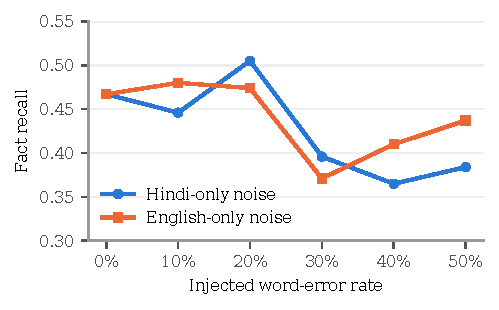
\includegraphics[width=\columnwidth]{figures/noise.pdf}}
\caption{Fact recall of English summaries as synthetic errors are injected only into Hindi or only into English words of the oracle transcript (0\% = oracle).}
\label{fig:noise}
\end{figure}

\subsection{Re-scripting is not mishearing}
Trelis's English-token error of 0.47 suggests heavy damage to English content. Aligning the oracle's 4,206 English words with the recogniser output shows that much of it is a change of script (Fig.~\ref{fig:enfate}): 52\% of English words are correct in Latin script, and 17\% appear in Devanagari with exactly the lexicon's spelling (\emph{click}~$\rightarrow$~\textit{klik} in Devanagari). Of the Devanagari substitutions that the lexicon can check, 75\% are exact re-scriptings. Counting those as correct lowers Trelis's English error to at most 0.31; extrapolating the same rate to unchecked words gives an estimate near 0.17. Transliterated WER does not capture this, because a romanised Devanagari spelling rarely matches the English spelling. The script-shift condition tests whether the summariser cares: writing 83\% of the oracle's English tokens in Devanagari leaves recall unchanged ($0.47 \rightarrow 0.48$, $p = 0.88$), and restoring Latin script in the Trelis output does not raise it ($0.44 \rightarrow 0.41$, $p = 0.43$). For this summariser, script variation in English terms is harmless, and standard WER overstates the downstream effect of a Hinglish recogniser.

\begin{figure}[t]
\centerline{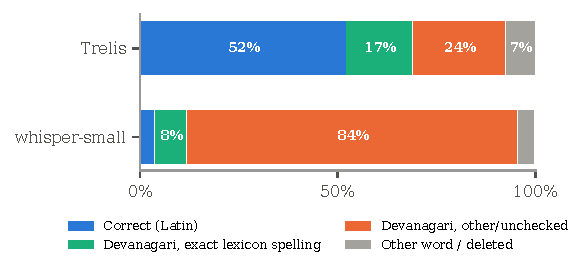
\includegraphics[width=\columnwidth]{figures/enfate.pdf}}
\caption{What each recogniser outputs for the 4,206 English words of the oracle transcripts. Much of Trelis's English ``error'' is a change of script rather than a misrecognition.}
\label{fig:enfate}
\end{figure}

\subsection{Adding on-screen text}\label{sec:screenres}
Table~\ref{tab:screen} and Fig.~\ref{fig:screen} give the screen results. In session A, raw screen text lowers recall from the oracle transcript by 0.12 (worse in 16 windows, better in 5; Holm $p = 0.015$) and from the Trelis transcript by 0.11 (Holm $p = 0.015$), and leaves whisper-small unchanged overall. The averages hide opposite effects by fact type. For whisper-small, facts visible on screen rise from 0.18 to 0.30 (+0.11, CI $[0.03, 0.20]$, better in 10 windows and worse in 2, uncorrected $p = 0.020$): the screen restores content that recognition lost. For the oracle, on-screen facts barely change (0.59 to 0.56) while speech-only facts fall from 0.46 to 0.31 (uncorrected $p = 0.016$). Summaries stay near 140 words, so screen text competes with speech for a fixed budget. Screen text alone recalls 0.11 of facts and only 0.04 of speech-only facts. Session B, judged separately, reproduces the raw-text loss for the oracle ($-0.12$, Holm $p = 0.043$).

Cleaning the OCR text cuts the oracle's loss to $-0.06$ (CI $[-0.16, 0.03]$, not significant); cleaned beats raw by 0.05 in 16 windows against 6, a consistent direction that is not significant ($p = 0.12$). For whisper-small, cleaned text keeps most of the on-screen gain (0.15 to 0.27, uncorrected $p = 0.025$) but lowers speech-only facts (0.20 to 0.10, uncorrected $p = 0.035$). OCR noise therefore explains part of the cost of screen text, but not all of it: even clean screen text shifts what the summary covers.

\begin{table*}[t]
\caption{Fact Recall with On-Screen Text (Window Means, 25 Windows). $\Delta$ Is the Paired Difference in Overall Recall from the Same Transcript without Screen Text, Judged in the Same Session.}
\label{tab:screen}
\centering
\footnotesize
\setlength{\tabcolsep}{5pt}
\begin{tabular}{llccccccc}
\toprule
Session & Input & Recall & On-screen f. & Speech-only f. & $\Delta$ recall & 95\% CI & Win/loss & Holm $p$ \\
\midrule
\multirow{7}{*}{A} & Oracle transcript & 0.514 & 0.594 & 0.459 & -- & -- & -- & -- \\
 & \quad + raw screen text & 0.392 & 0.556 & 0.314 & $-0.12$ & $[-0.20, -0.04]$ & 5/16 & 0.015 \\
 & Trelis ASR & 0.484 & 0.579 & 0.417 & -- & -- & -- & -- \\
 & \quad + raw screen text & 0.375 & 0.410 & 0.363 & $-0.11$ & $[-0.19, -0.04]$ & 4/14 & 0.015 \\
 & whisper-small ASR & 0.214 & 0.183 & 0.223 & -- & -- & -- & -- \\
 & \quad + raw screen text & 0.218 & 0.295 & 0.183 & $+0.00$ & $[-0.06, 0.08]$ & 9/10 & 0.62 \\
 & Raw screen text only & 0.114 & 0.200 & 0.044 & $-0.40^{\dagger}$ & $[-0.47, -0.33]$ & 0/24 & $<0.001$ \\
\midrule
\multirow{8}{*}{B} & Oracle transcript & 0.485 & 0.548 & 0.426 & -- & -- & -- & -- \\
 & \quad + raw screen text & 0.370 & 0.471 & 0.296 & $-0.12$ & $[-0.19, -0.04]$ & 6/18 & 0.043 \\
 & \quad + cleaned screen text & 0.423 & 0.494 & 0.339 & $-0.06$ & $[-0.16, 0.03]$ & 7/12 & 0.88 \\
 & whisper-small ASR & 0.194 & 0.148 & 0.195 & -- & -- & -- & -- \\
 & \quad + raw screen text & 0.204 & 0.298 & 0.163 & $+0.01$ & $[-0.05, 0.07]$ & 9/10 & 1.0 \\
 & \quad + cleaned screen text & 0.184 & 0.274 & 0.103 & $-0.01$ & $[-0.08, 0.05]$ & 10/8 & 1.0 \\
 & Trelis + cleaned screen text$^{\ddagger}$ & 0.389 & 0.442 & 0.341 & -- & -- & -- & -- \\
 & Cleaned screen text only & 0.119 & 0.172 & 0.061 & -- & -- & -- & -- \\
\bottomrule
\multicolumn{9}{p{0.92\textwidth}}{\scriptsize $^{\dagger}$ Relative to the oracle transcript. $^{\ddagger}$ Its no-screen counterpart was not re-judged in session B, so no test is reported. On-screen facts occur in 22 windows. Holm over the overall-recall rows of each session.}
\end{tabular}
\end{table*}

\begin{figure}[t]
\centerline{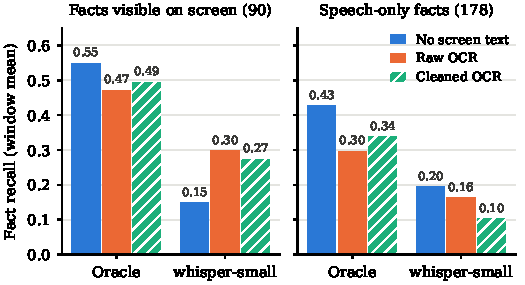
\includegraphics[width=\columnwidth]{figures/screen.pdf}}
\caption{Fact recall without screen text, with raw OCR text, and with cleaned OCR text, split by whether the fact is visible on screen (session B; window means). Screen text helps whisper-small on visible facts and costs speech-only facts; cleaning reduces the oracle's loss.}
\label{fig:screen}
\end{figure}

\subsection{Error patterns}
Recognition errors reach the summary as garbled product names: whisper-small heard ``gedit text editor'' as a Devanagari approximation, and the summary describes how to ``install and use Atit Text Editor''. Specific values are fragile: a fact stating that a compiled program prints ``total is 228'' is conveyed in all four oracle judging passes and in neither ASR condition. Even from the oracle transcript, the summariser often drops exact shortcuts and commands; the 31 facts built around a shortcut, command, path, or number have oracle recall 0.35 against 0.49 for other facts.

\subsection{Surface metrics}
ROUGE and BERTScore also detect the whisper-small loss (ROUGE-L $0.322 \rightarrow 0.246$; rescaled BERTScore $0.327 \rightarrow 0.247$; both Holm $p < 0.001$) and correlate moderately with fact recall across the 375 English summaries (Spearman $\rho$ = 0.54 and 0.46), but their scale is hard to interpret: recall halves while ROUGE-L falls by a quarter.

\subsection{Hinglish output}\label{sec:hinglish}
Asked for Hinglish, Qwen wrote mostly Devanagari Hindi (about 90\% of words). With 320 new tokens, 70 of 75 such summaries were cut off, because Devanagari needs several times more tokens per word; with 1,024 tokens, 68 of 75 ended cleanly and 6 fell into repetition loops. On the regenerated outputs, Hindi summaries of the oracle transcript recall 0.38 against 0.47 for English summaries ($p = 0.026$, CI $[-0.16, 0.01]$). The ASR pattern is the same as in English: whisper-small loses recall ($-0.18$, $p = 0.005$) and Trelis does not significantly ($-0.05$, $p = 0.16$). ROUGE-L against the English references is near 0.07 for these summaries, so surface metrics cannot compare across languages.

\section{Limitations}
The study is small: 25 windows from one domain (software tutorials) and only 28 English-tagged facts, so subgroup results are preliminary. References are silver, written by an LLM, although 97\% of checked facts were correct. A single summariser and a single judge model were used; the judge ran through a chat interface whose sampling settings cannot be controlled, and its test-retest agreement is moderate. The human validation used one annotator and 30 judge decisions. The language tag is a script-share rule; in the human check, 3 of the 5 sampled English-tagged facts were judged mixed. The two recognisers differ in size as well as in Hinglish fine-tuning. The oracle transcripts themselves are inconsistent in script for English words. For the screen conditions, 8 of 25 windows needed a weak or fallback alignment, OCR was English-only and read desktop text imperfectly, the on-screen fact split is a word-overlap heuristic computed from that OCR text, and the cleaning rules were set by hand (though frozen before use). Screen text was added to a fixed 120--180-word summary; a longer budget might change the trade-off.

\section{Conclusion}
For Hinglish tutorial videos, a generic small recogniser halves the factual content of LLM summaries, while a Hinglish-tuned recogniser causes no measurable loss, even though its word error rate, and especially its English-word error, suggest otherwise. Much of that error is English written in Devanagari, which the summariser handles without loss. Errors on Hindi words matter more than errors on English words at the same rate. On-screen text is a fallback rather than a free addition: it restores visible facts when recognition is poor but displaces spoken content when the transcript is good, and cleaning the OCR text reduces this cost without removing it. Future work should select only screen lines that the transcript does not already cover, let the summary budget grow with the input, fine-tune small recognisers on Hinglish speech, add human-written gold summaries and a second annotator, and test more summarisers and lecture domains.

% \section*{Acknowledgment}  % optional: uncomment and add text if needed

\section*{Disclosure of AI Use}
Silver reference summaries, atomic facts, and the initial English-to-Devanagari lexicon were generated with Gemini. Summaries were generated with Qwen2.5-7B-Instruct. Fact judgements were produced with Claude Sonnet 5.5. Analysis code and an initial draft of this paper were prepared with the assistance of Claude (Anthropic); the authors checked every number against the released results and take responsibility for the content. \todo{confirm this wording against the venue's AI policy}

\begin{thebibliography}{00}
\bibitem{diwan2021mucs} A. Diwan \textit{et al.}, ``MUCS 2021: Multilingual and code-switching ASR challenges for low resource Indian languages,'' in \textit{Proc. Interspeech}, 2021, pp. 2446--2450.
\bibitem{chadha2022} H. S. Chadha, P. Shah, A. Dhuriya, N. Chhimwal, A. Gupta, and V. Raghavan, ``Code switched and code mixed speech recognition for Indic languages,'' arXiv:2203.16578, 2022.
\bibitem{palaskar2019how2sum} S. Palaskar, J. Libovick\'{y}, S. Gella, and F. Metze, ``Multimodal abstractive summarization for How2 videos,'' in \textit{Proc. ACL}, 2019, pp. 6587--6596.
\bibitem{suresh2025cssum} S. K. Suresh, T. Surana, L. Z. Hao, and E. S. Chng, ``CS-Sum: A benchmark for code-switching dialogue summarization and the limits of large language models,'' in \textit{Proc. 5th New Frontiers in Summarization Workshop}, 2025, pp. 31--47.
\bibitem{mehnaz2021gupshup} L. Mehnaz \textit{et al.}, ``GupShup: Summarizing open-domain code-switched conversations,'' in \textit{Proc. EMNLP}, 2021, pp. 6177--6192.
\bibitem{radford2023whisper} A. Radford, J. W. Kim, T. Xu, G. Brockman, C. McLeavey, and I. Sutskever, ``Robust speech recognition via large-scale weak supervision,'' in \textit{Proc. ICML}, 2023.
\bibitem{trelis2025} Trelis Research, ``whisper-hinglish-preview,'' Hugging Face model card. [Online]. Available: \url{https://huggingface.co/Trelis/whisper-hinglish-preview} \todo{access date}
\bibitem{bhanushali2026csdi} K. Bhanushali and F. Hohl, ``An improved code-switching detection system for some Indic languages,'' in \textit{Proc. First Workshop on Multilingual Multicultural Evaluation}, 2026, pp. 35--48.
\bibitem{feng2021asrglue} L. Feng, J. Yu, D. Cai, S. Liu, H. Zheng, and Y. Wang, ``ASR-GLUE: A new multi-task benchmark for ASR-robust natural language understanding,'' arXiv:2108.13048, 2021.
\bibitem{binici2025medsage} K. Binici \textit{et al.}, ``MEDSAGE: Enhancing robustness of medical dialogue summarization to ASR errors with LLM-generated synthetic dialogues,'' in \textit{Proc. AAAI}, vol. 39, no. 22, 2025, pp. 23496--23504.
\bibitem{havare2026lost} J. Havare, A. Mittal, S. Tamilselvam, and G. Ramakrishnan, ``Lost in transcription: How speech-to-text errors derail code understanding,'' arXiv:2601.15339, 2026.
\bibitem{kumar2026ccic} V. D. Kumar, K. U. B. Reddy, and T. P. Karthik, ``An AI-powered framework for context-aware summarization of educational lectures,'' in \textit{Proc. Contemporary Computing Innovations Conf. (CCIC)}, Tirupati, India, 2026, pp. 1--6.
\bibitem{sanabria2018how2} R. Sanabria, O. Caglayan, S. Palaskar, D. Elliott, L. Barrault, L. Specia, and F. Metze, ``How2: A large-scale dataset for multimodal language understanding,'' in \textit{Proc. Workshop on Visually Grounded Interaction and Language (ViGIL), NeurIPS}, 2018.
\bibitem{smith2007tesseract} R. Smith, ``An overview of the Tesseract OCR engine,'' in \textit{Proc. 9th Int. Conf. Document Analysis and Recognition (ICDAR)}, 2007, pp. 629--633.
\bibitem{srivastava2021hinge} V. Srivastava and M. Singh, ``HinGE: A dataset for generation and evaluation of code-mixed Hinglish text,'' in \textit{Proc. 2nd Workshop on Evaluation and Comparison of NLP Systems}, 2021, pp. 200--208.
\bibitem{min2023factscore} S. Min \textit{et al.}, ``FActScore: Fine-grained atomic evaluation of factual precision in long form text generation,'' in \textit{Proc. EMNLP}, 2023, pp. 12076--12100.
\bibitem{zheng2023judge} L. Zheng \textit{et al.}, ``Judging LLM-as-a-judge with MT-Bench and Chatbot Arena,'' in \textit{Advances in Neural Information Processing Systems 36 (NeurIPS), Datasets and Benchmarks Track}, 2023.
\bibitem{lin2004rouge} C.-Y. Lin, ``ROUGE: A package for automatic evaluation of summaries,'' in \textit{Text Summarization Branches Out}, 2004, pp. 74--81.
\bibitem{zhang2020bertscore} T. Zhang, V. Kishore, F. Wu, K. Q. Weinberger, and Y. Artzi, ``BERTScore: Evaluating text generation with BERT,'' in \textit{Proc. ICLR}, 2020.
\bibitem{speer2022wordfreq} R. Speer, ``wordfreq,'' software library, v3.1. [Online]. Available: \url{https://github.com/rspeer/wordfreq}
\bibitem{qwen2025} A. Yang \textit{et al.} (Qwen Team), ``Qwen2.5 technical report,'' arXiv:2412.15115, 2024.
\bibitem{wilcoxon1945} F. Wilcoxon, ``Individual comparisons by ranking methods,'' \textit{Biometrics Bulletin}, vol. 1, no. 6, pp. 80--83, 1945.
\bibitem{holm1979} S. Holm, ``A simple sequentially rejective multiple test procedure,'' \textit{Scand. J. Statist.}, vol. 6, no. 2, pp. 65--70, 1979.
\bibitem{cohen1960} J. Cohen, ``A coefficient of agreement for nominal scales,'' \textit{Educ. Psychol. Meas.}, vol. 20, no. 1, pp. 37--46, 1960.
\end{thebibliography}

\end{document}
